\documentclass{beamer}

\usepackage[pantone3282,english]{wwustyle}

\usepackage[ngerman]{babel}
\usepackage[utf8]{inputenc}
\usepackage[T1]{fontenc}

\usepackage{color}
\definecolor{eclipseBlue}{RGB}{42,0.0,255}
\definecolor{eclipseGreen}{RGB}{63,127,95}
\definecolor{eclipsePurple}{RGB}{127,0,85}
\usepackage{listings}
\lstdefinelanguage{htsi}{%
	keywords={for, in, to, if, else, ifEnd, forEnd, True, False},%
	ndkeywords={random, get, set, wait},%
	sensitive=false,%
	morecomment=[l]{#}%
}
\lstset{%
	language={htsi},%
	basicstyle=\scriptsize\ttfamily, % Global Code Style
	captionpos=b, % Position of the Caption (t for top, b for bottom)
	extendedchars=true, % Allows 256 instead of 128 ASCII characters
	tabsize=2, % number of spaces indented when discovering a tab 
	columns=fixed, % make all characters equal width
	keepspaces=true, % does not ignore spaces to fit width, convert tabs to spaces
	showstringspaces=false, % lets spaces in strings appear as real spaces
	breaklines=true, % wrap lines if they don't fit
	%frame=trbl, % draw a frame at the top, right, left and bottom of the listing
	%frameround=tttt, % make the frame round at all four corners
	%framesep=4pt, % quarter circle size of the round corners
	numbers=left, % show line numbers at the left
	xleftmargin=1em,%
	numberstyle=\tiny\ttfamily, % style of the line numbers
	commentstyle=\color{eclipseGreen}, % style of comments
	keywordstyle=\color{eclipsePurple}, % style of keywords
	ndkeywordstyle=\color{eclipseBlue},
	%stringstyle=\color{eclipseBlue} % style of strings
}

\usepackage{graphicx}
\usepackage{pgfplots}
\usepackage{tikz}
\tikzset{font=\tiny}
\usetikzlibrary{positioning,decorations.pathreplacing,shapes, automata}

% Uncomment the following two lines if you want to prepare your document for
% the fast mode.
% \usetikzlibrary{external}
% \tikzexternalize

\author{Christof, Marius, Thomas}
\title{IT-Security in smart grids}
%\institutelogo{Logo on title frame}
%\institutelogosmall{Logo on other frames}
\subtitle{Defence strategies for Remote Terminal Units in SCADA networks with limited communication}

\begin{document}

%%%%%%%%%%%%%%% WWUstyle "fast" mode %%%%%%%%%%%%%%%%%%%%%
% Do the following steps in order to speed up the compilation time of your
% presentation:
%
% 1. Include the externalization tikz library in the preamble of your document.
%    This is always recommended if you are using tikz in your document.
% 2. Uncomment the \wwupreparefastmode command below
% 3. Compile your document with command line option '-shell-escape',
%    e.g.: 'pdflatex -shell-escape beamer.tex'
% 4. Comment (or delete) the \wwupreparefastmode
% 5. Add option 'fast' to the 'wwustyle' package declaration line.
% 6. Be happy!

% \wwupreparefastmode


\begin{frame}[plain]
	\maketitle
\end{frame}

\begin{frame}
	\frametitle{Table of contents}
	\begin{itemize}
		\item The Scenario
		\pause
		\item Implementation in mosaik
			\begin{itemize}
				\item Topology Loader
				\item RTU Simulation
				\item Intrusion Detection System
				\item WebVis
				\item Hacker Tools
				\item Operator Tools
			\end{itemize}
		\pause
		\item Attack Scenarios
			\begin{itemize}
				\item Deterministic attacks
				\item Random attacks
				\item Defence mechanism specialized attacks
				\item Attack to kill the IDS
			\end{itemize}
	\end{itemize}
\end{frame}

\begin{frame}
	\frametitle{Table of contents}
	\begin{itemize}
		\item Discussion
			\begin{itemize}
				\item Evaluation
				\item Conclusion
				\item Future work
			\end{itemize}
	\end{itemize}
\end{frame}

\begin{frame}
	\frametitle{The Scenario}
	\centering
	Topologie 1 and 1a \\
	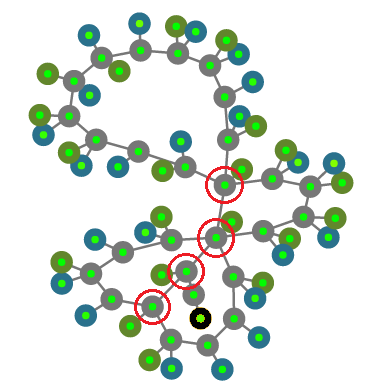
\includegraphics[height=0.8\textheight]{pics/topo_1_2.png}
\end{frame}

\begin{frame}
	\frametitle{The Scenario}
	\centering
	Topologie 2 \\
	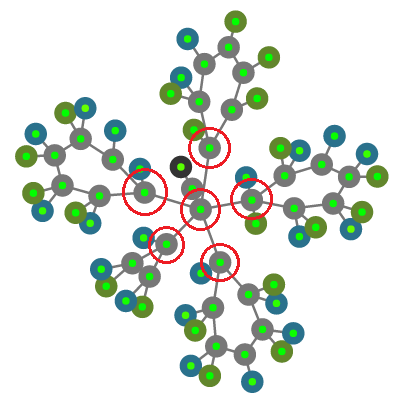
\includegraphics[height=0.8\textheight]{pics/topo_3.png}
\end{frame}

\begin{frame}
	\frametitle{The Scenario}
	\centering
	Topologie 3 and 3a \\
	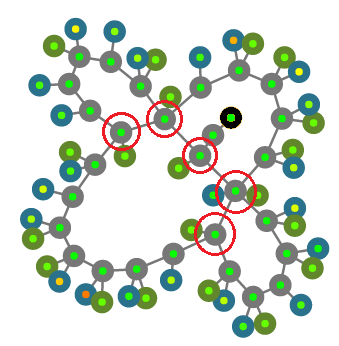
\includegraphics[height=0.8\textheight]{pics/topo_4_4a.png}
\end{frame}

\begin{frame}
	\frametitle{The Scenario}
	\centering
	Topologie 4 \\
	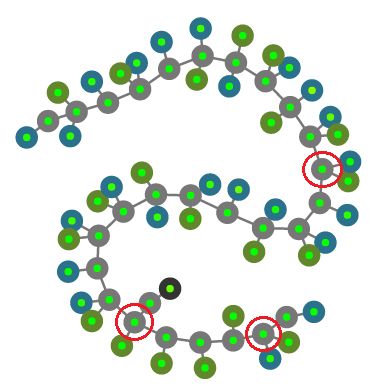
\includegraphics[height=0.8\textheight]{pics/topo_5.png}
\end{frame}

\begin{frame}
	\frametitle{The Scenario}
	\centering
	Topologie 5 \\
	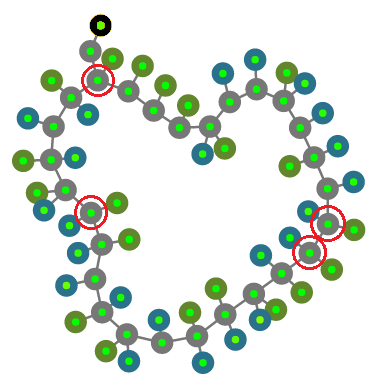
\includegraphics[height=0.8\textheight]{pics/topo_6.png}
\end{frame}

\begin{frame}
	\frametitle{Implementation in mosaik}
	\begin{figure}
		\begin{tikzpicture}[auto, node distance=1cm and 2cm]
		\tikzstyle{class} = [rectangle, draw=black, thick, align=center];
		\tikzstyle{start} = [align=center];
		
		\node[class](topology loader){Topology \\ Loader};
		\node[start, left = of topology loader](start1){};
		\node[class, below = of topology loader](operator){Operator \\ Tools};
		\node[class, below = of operator](simulation){Simulation};
		\node[class, right = of simulation](webvis){Web \\ Visualisation};
		\node[class, below = of webvis](topologysim){Topology \\ simulation};
		\node[class, above = of webvis](RTUsim){RTU \\ simulations};
		\node[class, left = of topologysim](pypower){PyPower};
		\node[class, right = of RTUsim](hackertools){Hacker \\ Tools};
		\node[class, above = of hackertools](hackercmd){Hacker \\ CMD};
		\node[start, left = of hackercmd](start2){};
		\node[class, below = of hackertools](htsi){Hacker Tools \\ Script Interpreter};
		
		\path[draw=black, thick, ->] (topology loader) edge node{starts} (operator)
		(operator) edge node{starts} (simulation)
		(simulation) edge node{manages} (RTUsim)
		(simulation) edge node{manages} (webvis)
		(simulation) edge node{manages} (topologysim)
		(simulation) edge node{manages} (pypower)
		(hackertools) edge node{uses} (htsi)
		(start1) edge node{run} (topology loader)
		(start2) edge node{run} (hackercmd);
		
		\path[draw=red, thick, <->] (RTUsim) edge node{communicates} (hackertools)
		(RTUsim) edge node{communicates} (operator)
		(RTUsim) edge node{communicates} (webvis)
		(RTUsim) edge [loop above] node{communicates} (RTUsim)
		(hackertools) edge node{communicates} (hackercmd)
		(hackertools) edge node{communicates} (webvis);
		\end{tikzpicture}
	\end{figure}
\end{frame}

\begin{frame}
	\frametitle{Implementation in mosaik}
	\begin{itemize}
		\item Topology Loader
			\begin{itemize}
				\item provides a GUI
				\item image of topology selected
				\item some simulation configuration
			\end{itemize}
		\pause
		\item RTU Simulation
			\begin{itemize}
				\item one main MonitoringRTU
				\item handles the individual RTU simulations running in separate threads
				\item passes data between mosaik and the RTUs
				\item RTUs can communicate via server object
			\end{itemize}
	\end{itemize}
\end{frame}

\begin{frame}
	\frametitle{Implementation in mosaik}
	\begin{itemize}
		\item Intrusion Detection System
			\begin{itemize}
				\item behaviour specification based
				\pause
				\item regulation
					\begin{itemize}
						\item turn of branch when max current is exceeded
						\item cut-off values to turn secondary branches on/off
					\end{itemize}
				\pause
				\item validation
					\begin{itemize}
						\item general system \\
								\quad - trusted and untrusted sensors \\
								\quad - warning value \\
								\quad - warnings and great warnings \\
						\item specific checks \\
								\quad - Kirchhoff's Law \\
								\quad - voltage within 10\% of expected voltage \\
								\quad - realistic physical value change
					\end{itemize}
			\end{itemize}
	\end{itemize}
\end{frame}

\begin{frame}
	\frametitle{Implementation in mosaik}
	\begin{itemize}
		\item Intrusion Detection System
		\begin{itemize}
			\item validation
				\begin{itemize}
					\item specific checks \\
							\quad - voltage angle difference between two nodes not too big \\
							\quad - check if all sensor values at a node are the same for \\ \quad \space \space voltage angle and voltage magnitude \\
								\qquad + majority rule \\
								\qquad + mistrust every sensor
				\end{itemize}
		\end{itemize}
	\end{itemize}
\end{frame}

\begin{frame}
	\frametitle{Implementation in mosaik}
	\begin{itemize}
		\item WebVis
			\begin{itemize}
				\item switched from executable to Python script
				\item added visualisation of attacks and RTU interventions
			\end{itemize}
		\pause
		\item Hacker Tools
			\begin{itemize}
				\item Hacker Tools CMD
					\begin{itemize}
						\item simple command line shell
						\item manipulate sensor data or change switch states
						\item TCP communication with RTUs' servers and WebVis
					\end{itemize}
				\pause
				\item Hacker Tools Script Interpreter
					\begin{itemize}
						\item automating attacks through scripts
						\item self-developed script language
					\end{itemize}
			\end{itemize}
	\end{itemize}
\end{frame}

\begin{frame}
	\frametitle{Implementation in mosaik}
	\begin{itemize}
		\item Hacker Tools Script Interpreter
			\begin{itemize}
				\item set and get for variables
				\item if - then - else
				\item for-loop
					\begin{itemize}
						\item over a range of values
						\item over an array
					\end{itemize}
				\item random-function
					\begin{itemize}
						\item number in range
						\item element from array
					\end{itemize}
				\item array length function
				\item wait function (waits a given amount of seconds)
			\end{itemize}
	\end{itemize}
\end{frame}

\begin{frame}
	\frametitle{Implementation in mosaik}
	\lstinputlisting{scripts/increaseall.txt}
\end{frame}

\begin{frame}
	\frametitle{Implementation in mosaik}
	\lstinputlisting{scripts/randomrtu.txt}
\end{frame}

\begin{frame}
	\frametitle{Implementation in mosaik}
	\begin{itemize}
		\item Operator Tools
			\begin{itemize}
				\item simple GUI showing RTU attack warning messages
				\item button to reset RTUs' trust-label
			\end{itemize}
	\end{itemize}
\end{frame}

\begin{frame}
	\frametitle{Attack Scenarios}
	\begin{itemize}
		\item Deterministic attacks
			\begin{itemize}
				\item easy to implement
				\item predetermined sequence of commands
			\end{itemize}
		\pause
		\item Random attacks
			\begin{itemize}
				\item no pattern
				\item tries to circumvent pattern recognition
			\end{itemize}
		\pause
		\item Defence mechanism specialized attacks
			\begin{itemize}
				\item Kirchhoff's Law
				\item mimic natural gradients
				\item and more
			\end{itemize}
	\end{itemize}
\end{frame}

\begin{frame}
	\frametitle{Attack Scenarios}
	\begin{itemize}
		\item Attack to kill the IDS
			\begin{itemize}
				\item heavy attack $\rightarrow$ IDS declares all sensors as unsafe
				\item grid is not controlled any more
				\item can reach unsafe states on its own without the IDS noticing
			\end{itemize}
	\end{itemize}
\end{frame}

\begin{frame}
	\frametitle{Discussion}
	\begin{itemize}
		\item Evaluation
			\begin{itemize}
				\item sensor value logging
				\item specific and random attack
				\item executed on topology 1
			\end{itemize}
	\end{itemize}
\end{frame}

\begin{frame}
	\frametitle{Discussion}
	\begin{itemize}
		\item Specific attack \\
			\begin{tikzpicture}
				\begin{axis}[height=0.9\textheight, xlabel={time [t]}, ylabel={I\_real [A]}, legend style={font=\fontsize{6}{6}\selectfont}]
					\addplot table [y=sensor_2, mark=none] {stats/topo1/normal/I_real_all.txt};
					\addplot table [y=sensor_2, mark=none] {stats/topo1/spec/I_real_all.txt};
					\addplot table [y=sensor_4, mark=none] {stats/topo1/normal/I_real_all.txt};
					\addplot table [y=sensor_4, mark=none] {stats/topo1/spec/I_real_all.txt};
					\legend{{sensor 2, normal}, {sensor 2, attack}, {sensor 4, normal}, {sensor 4, attack}}
				\end{axis}
			\end{tikzpicture}
	\end{itemize}
\end{frame}

\begin{frame}
	\frametitle{Discussion}
	\begin{itemize}
		\item Random attack \\
			\begin{tikzpicture}
				\begin{axis}[height=0.9\textheight, xlabel={time [t]}, ylabel={I\_real [A]}]
					\addplot table [y=sensor_1, mark=none] {stats/topo1/rand/I_real_all.txt};
					\addplot table [y=sensor_2, mark=none] {stats/topo1/rand/I_real_all.txt};
					\addplot table [y=sensor_3, mark=none] {stats/topo1/rand/I_real_all.txt};
					\addplot table [y=sensor_4, mark=none] {stats/topo1/rand/I_real_all.txt};
					\addplot table [y=sensor_5, mark=none] {stats/topo1/rand/I_real_all.txt};
					\addplot table [y=sensor_6, mark=none] {stats/topo1/rand/I_real_all.txt};
					\addplot table [y=sensor_7, mark=none] {stats/topo1/rand/I_real_all.txt};
					\addplot table [y=sensor_8, mark=none] {stats/topo1/rand/I_real_all.txt};
					\addplot table [y=sensor_9, mark=none] {stats/topo1/rand/I_real_all.txt};
					\addplot table [y=sensor_10, mark=none] {stats/topo1/rand/I_real_all.txt};
					\addplot table [y=sensor_11, mark=none] {stats/topo1/rand/I_real_all.txt};
					\addplot table [y=sensor_12, mark=none] {stats/topo1/rand/I_real_all.txt};
					\addplot table [y=sensor_13, mark=none] {stats/topo1/rand/I_real_all.txt};
					\addplot table [y=sensor_14, mark=none] {stats/topo1/rand/I_real_all.txt};
					\addplot table [y=sensor_15, mark=none] {stats/topo1/rand/I_real_all.txt};
					\addplot table [y=sensor_16, mark=none] {stats/topo1/rand/I_real_all.txt};
					\addplot table [y=sensor_17, mark=none] {stats/topo1/rand/I_real_all.txt};
					%\legend{1, 2, 3, 4, 5, 6, 7, 8, 9, 10, 11, 12, 13, 14, 15, 16, 17}
				\end{axis}
			\end{tikzpicture}
	\end{itemize}
\end{frame}

\begin{frame}
	\frametitle{Discussion}
	\begin{itemize}
		\item Conclusion
			\begin{itemize}
				\item Kirchhoff's Law is hard to trick
					\begin{itemize}
						\item many false positives if a sensor on a node is attacked
						\item consider majority rule for improvement
					\end{itemize}
				\item overall very accurate attack detection
				\item low number of false positives
			\end{itemize}
	\end{itemize}
\end{frame}

\begin{frame}
	\frametitle{Discussion}
	\begin{itemize}
		\item Future Work
			\begin{itemize}
				\item consider that current decreases in in the grid
				\item more extensive command validation
				\item take current readings of PVs and houses into account
				\item testing if supplementary pattern based attack recognition would be useful
				\item maybe add rules to restore the trust of a sensor
				\item syntax error checks for script interpreter
			\end{itemize}
	\end{itemize}
\end{frame}

\begin{frame}
	\centering
	Demonstration
\end{frame}

\begin{frame}
	\centering
	Thank you for your attention! \\
	Any questions?
\end{frame}

\end{document}
